%
% latex-sample.tex
%
% This LaTeX source file provides a template for a typical research paper.
%

%
% Use the standard article template.
%
\documentclass[100pt]{article}

% The geometry package allows for easy page formatting.
\usepackage{geometry}
\geometry{letterpaper}

% Load up special logo commands.
\usepackage{doc}

% Package for formatting URLs.
\usepackage{url}

% Packages and definitions for graphics files.
\usepackage{graphicx}
\usepackage{epstopdf}
\DeclareGraphicsRule{.tif}{png}{.png}{`convert #1 `dirname #1`/`basename #1 .tif`.png}

%
% Set the title, author, and date.
%
\title{\Large{Assignment 1210}}
\author{\Large{Mondo Yamaguchi}}
\date{\Large{12/10/2015}}

%
% The document proper.
%
\begin{document}

% Add the title section.
\maketitle


\section{\Large{Concept}}
\large{
I have put together a front end for the LMU Diabolical web service for my dream interface. The diabolical simulates a hypothetical role-playing game backed by Google App Engine. For this very simple web service, I have implemented five non-trivial functions: Display a list of current characters, create a new character, view a character, modify a character and delete a character. 
}

\section{\Large{Description of the five functions}}
\large{
For the display of a characters list function, I put the list into a table that utilizes striped rows to add zebra-striping. When the user presses the show button, the table pops up on the screen. Because of zebra-striping, the user can easily see each character's six identities (character ID, name, gender, level, class type, and money). There is also the hide button to put the table away. For the creating a new character function, I built six boxes for each of a character's identities and placed the create button. The box has two labels, one on the top of the box and the other inside the box, to make sure the user does not make a mistake while he/she inputs character's identities. The box flashes once the user presses it, which is an important feature of this component to improve the user's efficiency and minimize the user's error. After the user inputs a character's identities, the user can click the create button to generate the new character, and the user gets an alert that shows information of the new character. For the view a character function, the user can search a character by a character's id and gets a table of the specific character the user wants. I implemented a box for the input of a character's id and two boxes for displaying and hiding the user's search result. The interface for the modifying a character function looks the same as the create a new character function. This function modifies a character's identities instead of creating a new character. Similarly, the interface for the deleting a character function looks the same as the viewing a character function. This function instead delete a character. Lastly, the spawn a random item function generates a new random character. I have two input boxes and the spawn button. When the user inputs a level and a slot and presses the spawn button, the function creates a random character.
\\\\
In addition, when the user hovers over any buttons, it triggers an action that let the user know he/she can press the button. 

\section{\Large{Layout}}
\large{
The overall structure of the interface is very simple. It has plain white background and black labels for green buttons and white boxes. Everything is centered in the middle of the page, and all of the buttons are colored in same color so that the user can easily notice it. 
}\\\\\\\\\\\\\\\\\\\\\\\\\\\\\\\\\\\\\\\\\\\\\\\\\\\

\begin{figure}[h!]
\hspace*{2.2cm} 
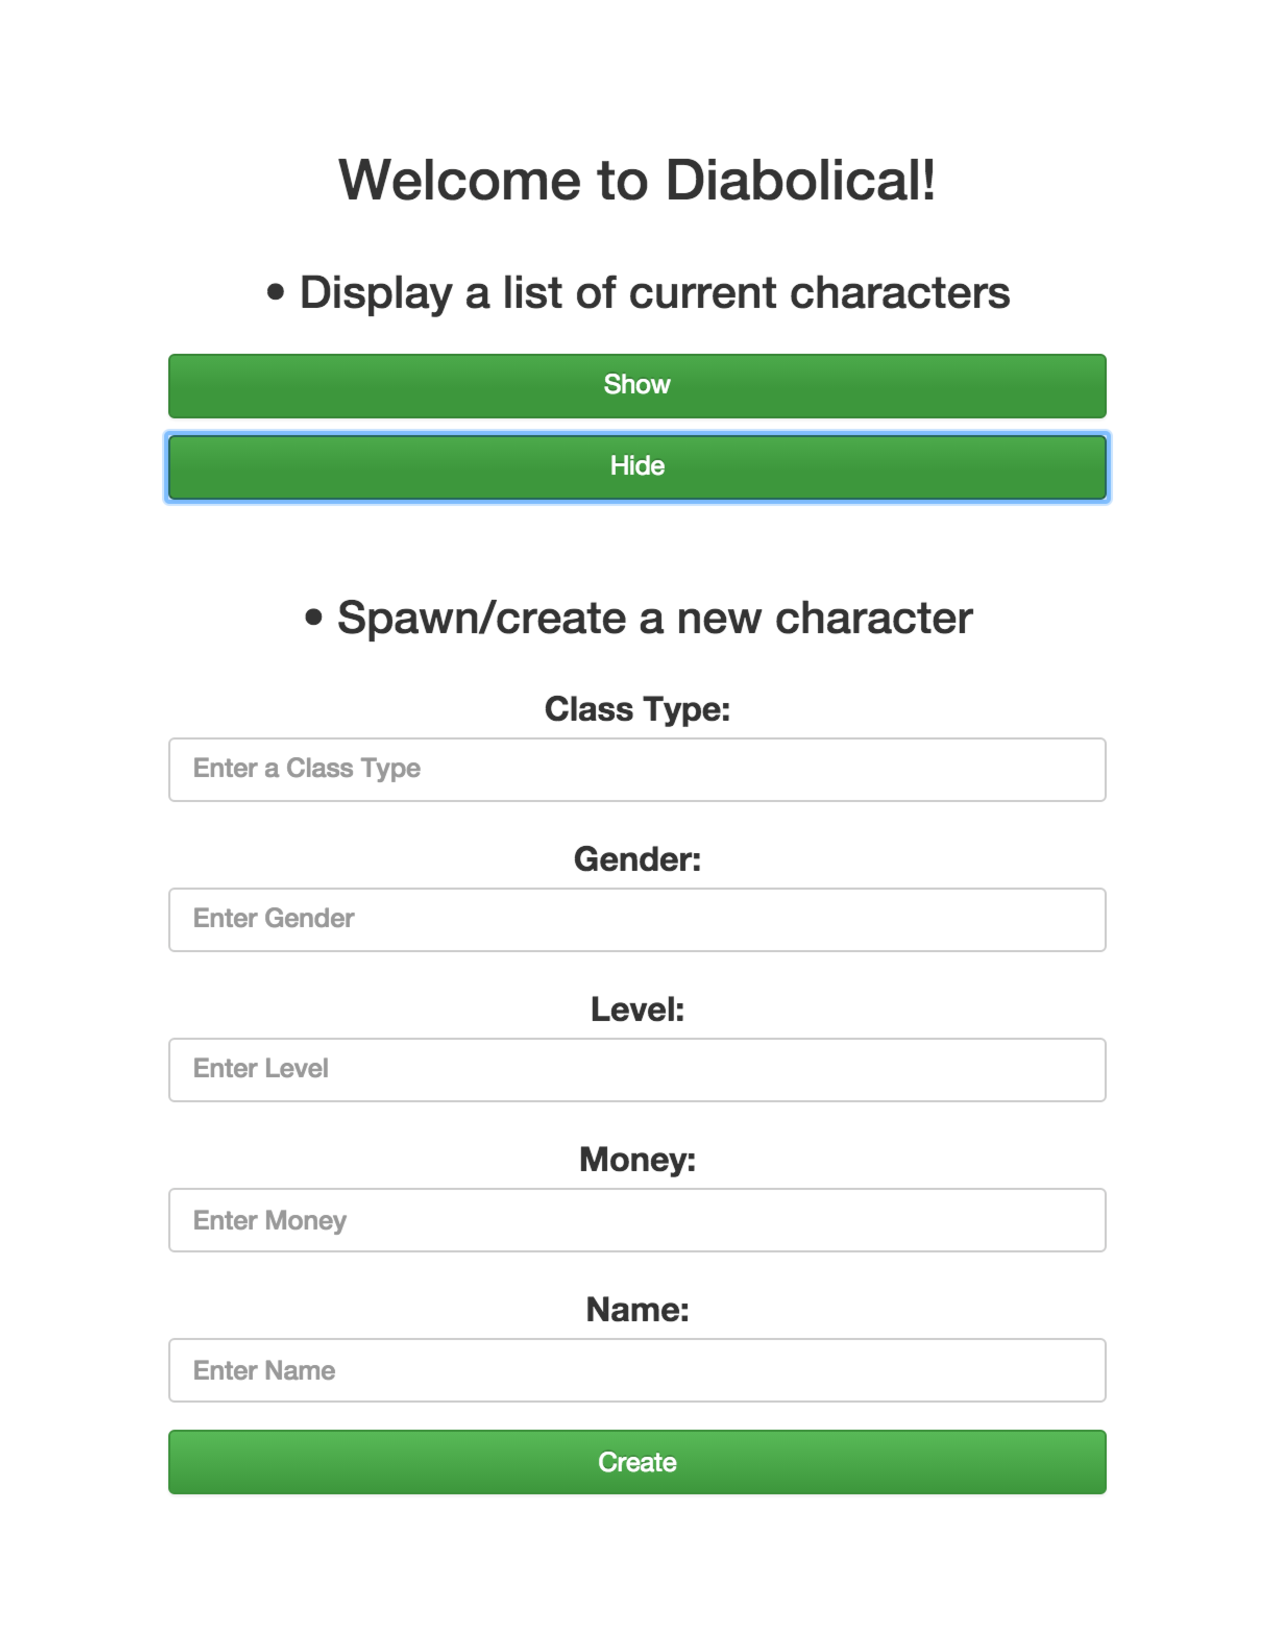
\includegraphics[width=0.84cm, natwidth=50,natheight=10]{1.pdf}
\end{figure}

\section{ Two usage Scenarios}
\subsection{Creating a new character and viewing it on the table}
\large{
The user can create a new character by inputing his/her character's information into the create a new character function. After the user presses the create button, he/she can see the new character on the characters list by clicking the show button of the displaying of a characters list function. 
}
\subsection{Search a character and delete}
\large{
The user can search any character on the list by inputing a character ID into the view a character function. Then, he/she can delete a character by putting a character ID into the deleting a character function and hitting the delete button. 
}

\section{Principle}
I have utilized Ben Shneiderman's "Eight Golden Rules of Interface Design" as a guide in order to develop my front end for the Diabolical web service. The interface only contains two types of component and only one type of input box and button are used to keep its consistency (Strive for consistency). Every button reacts when the user hover over them (Offer informative feedback) and it gives an alert each time the user plays an action to confirm what he/she has done (Design dialog to yield closure). The modifying a character and the deleting a character functions let the user to change or delete a character in case he/she unintentionally created a character (Offer simple error handling). Finally, all the functions are kept simple for the user (Reduce short-term memory load).

\section{Conclusion}
My design's strong metrics are learnability, efficiency, errors, and memorability because I have tried to keep my front end for the LMU Diabolical web service as simple as possible and utilized Ben Shneiderman's "Eight Golden Rules of Interface Design" as a guide. However, the weak metric would be satisfaction since it provides only five functions and all of them are not entertaining and not exciting. 
\pagebreak

\begin{thebibliography} {1}
http://myweb.lmu.edu/dondi/share/ixd/principles.pdf
\end{thebibliography}

\end{document}